\documentclass[cyan]{elegantnote}
\author{Yuyang Songsheng}
\email{songshengyuyang@gmail.com}
\zhtitle{物理}
\entitle{Physics}
\version{1.00}
\myquote{Do not ask what it is. Ask what you can say about it.}
\logo{logo.jpg}
\cover{cover.pdf}
%green color
   \definecolor{main1}{RGB}{210,168,75}
   \definecolor{seco1}{RGB}{9,80,3}
   \definecolor{thid1}{RGB}{0,175,152}
%cyan color
   \definecolor{main2}{RGB}{239,126,30}
   \definecolor{seco2}{RGB}{0,175,152}
   \definecolor{thid2}{RGB}{236,74,53}
%cyan color
   \definecolor{main3}{RGB}{127,191,51}
   \definecolor{seco3}{RGB}{0,145,215}
   \definecolor{thid3}{RGB}{180,27,131}


\usepackage{makecell}
\usepackage{lipsum}
\usepackage{amssymb}
\usepackage{float}
\usepackage{wrapfig}
\usepackage{latexsym}
\usepackage{hyperref}
\usepackage{feynmf}
\usepackage{exscale}
\usepackage{relsize}
\usepackage{bm}%bold math, for vector


\begin{document}
\maketitle
\tableofcontents
\chapter{Angular Momentum}
\section{Eigenvalues of angular momentum operator}
The commutation relations among the angular momentum operators are
\[[J_i,J_j] = \epsilon_{ijk} J_k\]
And these three operators are self-adjoint. We first introduce the operator $J^2 = J_x^2 + J_y^2 + J_z^2$. We can verify that $[J^2,\bm{J}] = 0$. Thus there exists a complete set of common eigenvectors of $J^2$ and any one component of $\bm{J}$. Particularly, we have the pair of eigenvalue equations
\[J^2 | \beta,m\rangle = \beta | \beta,m\rangle \quad J_z | \beta,m\rangle = m | \beta,m\rangle\]
Since
\[\langle \beta,m | J^2 | \beta,m \rangle = \langle \beta,m | J_x^2 | \beta,m \rangle + \langle \beta,m | J_y^2 | \beta,m \rangle + \langle \beta,m | J_z^2 | \beta,m \rangle\]
we have $m^2 \leq \beta$. Thus for a fixed value of $\beta$ there must be maximum and minimum values for $m$.\\
Define
\[J_+ \equiv J_x + iJ_y \quad J_- \equiv J_x - iJ_y\]
we have the commutation relations
\[[J_z,J_+] = J_+ \quad [J_z,J_-] = -J_- \quad [J_+,J_-] = 2J_z\]
So
\[J_z J_+ | \beta,m\rangle = J_+(J_z + 1)| \beta,m\rangle = (m+1)J_+| \beta,m\rangle\]
Therefore, either $J_+ | \beta,m\rangle$ is an eigenvector of $J_z$ with the raised eigenvalue $m+1$, or $J_+ | \beta,m\rangle = 0$. Now for fixed $\beta$ there is a maximum value of $m$, which we shall denote as $j$. It must be the case that
\[J_+ |\beta,j\rangle = 0\]
Since
\[J_- J_+ = J^2 - J_z^2 - J_z\]
it is obvious that $\beta = j(j+1)$. By similar method, we can show the minimum eigenvalue of $J_z$ for fixed $\beta$ satisfy that $\beta = k(k-1)$. So, we have $k = -j$. \\
We have thus shown the existence of a set of eigenvectors corresponding to integer spaced $m$ values in the range $-j \leq m \leq j$. Since the difference between the maximum value $j$ and the minimum value $-j$ must be an integer, it follows that $j = \mbox{ integer} / 2$. Henceforth we shall adopt the common and more convenient notation of labeling the eigenvectors by $j$ instead of by $\beta$. Thus the vector that was previously denoted as $|\beta,m\rangle$ will now be denoted as $|j,m\rangle$. \\ \\
To find the matrix element of angular momentum operator, we notice that
\[\langle j,m| J_-J_+|j,m\rangle = j(j+1)-m(m+1)\]
so, we can get
\[J_+ |j,m\rangle = \sqrt{(j+m+1)(j-m)} |j,m+1\rangle\]
Similarly, we have
\[J_- |j,m\rangle = \sqrt{(j-m+1)(j+m)} |j,m-1\rangle\]
The matrix element of $J_+$, $J_-$ and $J_z$ are
\[\langle j',m'| J_+ | j,m\rangle = \sqrt{(j+m+1)(j-m)} \delta_{jj'}\delta_{m',m+1}\]
\[\langle j',m'| J_- | j,m\rangle = \sqrt{(j-m+1)(j+m)} \delta_{jj'}\delta_{m',m-1}\]
\[\langle j',m'| J_z | j,m\rangle = m \delta_{jj'}\delta_{m',m}\]

\section{Orbital Angular Momentum and Spin}
Let $\psi(\bm{x})$ be a one-component state function in coordinate representation. When it is subjected to a rotation it is transformed into
\[\bm{R}\psi(\bm{x}) = \psi(R^{-1}\bm{x})\]
where $\bm{R}$ is the rotation operator generated by $\bm{R} = \exp(-i\bm{J}\cdot\bm{n}\theta)$. For a rotation through infinitesimal angle $\epsilon$ about the $z$ axis, we have
\[\bm{R}_z(\epsilon) \psi(x,y,z) = \psi(x+\epsilon y,y-\epsilon x,z) = \psi(x,y,x) + \epsilon (y \frac{\partial \psi}{\partial x} - x \frac{\partial \psi}{\partial y})\]
On the other hand, 
\[\bm{R}_z(\epsilon) = I - i\epsilon J_z\]
so, we have $J_z = -i(x \frac{\partial}{\partial y} - y \frac{\partial}{\partial x})$. This is just the $z$ component of the orbital angular momentum operator $L = \bm{X} \times \bm{P}$.\\
For a multicomponent state function, we have
\[\bm{R} \left( \begin{matrix} \psi_1(\bm{x}) \\ \psi_2(\bm{x}) \\  \vdots \end{matrix} \right) = D \left( \begin{matrix} \psi_1(R^{-1}\bm{x}) \\ \psi_2(R^{-1}\bm{x}) \\  \vdots \end{matrix} \right)\]
Thus the general form of the rotation operator will be
\[\bm{R}_{n}(\theta) = e^{-i\bm{L}\cdot\bm{n}\theta}D_n(\theta)\]
The two factors commute because the first acts only on the coordinate and the second acts only on the components of the column vector. The matrix $D$ must be unitary, and so it can be written as
\[D_n(\theta) = e^{-i\bm{S}\cdot\bm{n}\theta}\]
The angular momentum operator $\bm{J}$ has the form
\[\bm{J} = \bm{L} + \bm{S}\]
with $\bm{L} = \bm{X} \times \bm{P}$ and $[L_{\alpha},S_{\beta}] = 0$. In the particular representation used in this section, we have $\bm{L} = -i\bm{x}\times\bm{\nabla}$, and the components of $S$ are
discrete matrices. The operators $\bm{L}$ and $\bm{S}$ are called the orbital and spin parts of the angular momentum.
\subsubsection{Orbital angular momentum}
The form of the gradient operator in spherical coordinates is
\[\bm{\nabla} = \bm{e}_r \frac{\partial}{\partial r} + \bm{e}_{\theta} \frac{1}{r} \frac{\partial}{\partial \theta} + \bm{e}_{\phi} \frac{1}{r\sin\theta} \frac{\partial}{\partial \phi}\]
The orbital angular momentum operator then has the form
\[\bm{L} = r\bm{e}_r \times (-i\bm{\nabla}) = (-i) \left[ \bm{e}_{\phi} \frac{\partial}{\partial \theta} - \bm{e}_{\theta} \frac{1}{\sin\theta} \frac{\partial}{\partial \phi} \right]\]
So,we have
\[L_z = \bm{L}\cdot\bm{e}_z = -i\frac{\partial}{\partial \phi}\]
\[L^2 = \bm{L}\cdot\bm{L} = - \left [ \frac{1}{\sin\theta} \frac{\partial }{\partial \theta} (\sin\theta \frac{\partial }{\partial \theta}) + \frac{1}{\sin^2\theta} \frac{\partial^2}{\partial \phi^2}  \right ]\]
We must now solve the two coupled differential equations,
\[L_z Y(\theta,\phi) = m Y(\theta,\phi) \quad L^2 Y(\theta,\phi) = l(l+1) Y(\theta,\phi)\]
Apart from normalization, we have $Y(\theta,\phi) = e^{im\phi}P_l^m(\cos\theta)$. Here, $P_l^m$ is the \href{https://en.wikipedia.org/wiki/Associated_Legendre_polynomials}{associated Legendre polynomials}. If we assume that the solution must be single-valued under rotation, then it will follow that $m$ must be an integer. If we further assume that it must be nonsingular at $\theta = 0$ and $\theta = \pi$, then from the standard theory of the Legendre equation it will follow that $l$ must be a nonnegative integer in the range $l \geq |m|$. The normalized solutions that result from these assumptions are the well-known \href{https://en.wikipedia.org/wiki/Spherical_harmonics}{spherical harmonics}
\[Y_l^m(\theta,\phi) = (-1)^{(m+|m|)/2} \left [\frac{(2l+1)(l-|m|)!}{4\pi(l+|m|)!}  \right ]^{1/2}e^{im\phi} P_l^{|m|}(\cos\theta)\]
\subsubsection{Spin}
A particular species of particle is characterized by a set of quantum numbers that includes the value of its spin s, it is often sufficient to treat the spin operators $\bm{S}$ as acting on the space of dimension
$2s+1$ that is spanned by the eigenvectors of for a fixed value of $s$. \\
If $s= \frac{1}{2}$, we have
\[S_x = \frac{1}{2} \left[ \begin{matrix} 0& 1\\ 1& 0\end{matrix} \right] \quad S_y = \frac{1}{2} \left[ \begin{matrix} 0& -i\\ i& 0\end{matrix} \right] \quad S_z = \frac{1}{2} \left[ \begin{matrix} 1& 0\\ 0& -1\end{matrix} \right]\]
The spin operator in direction $\bm{n} = (\sin\theta\cos\phi,\sin\theta\sin\phi,\cos\theta)$ is
\[\bm{S}_{n} = \frac{1}{2} \left[ \begin{matrix} \cos\theta& e^{-i\phi}\sin\theta\\ e^{i\phi}\sin\theta& -\cos\theta\end{matrix} \right]\]
The eigenvectors are
\[\left[ \begin{matrix} e^{-i\phi/2}\cos\frac{\theta}{2}\\ e^{i\phi/2}\sin\frac{\theta}{2} \end{matrix} \right] \quad \left[ \begin{matrix} -e^{-i\phi/2}\sin\frac{\theta}{2}\\ e^{i\phi/2}\cos\frac{\theta}{2} \end{matrix} \right]\]
corresponding to eigenvalues $\frac{1}{2}$ and $-\frac{1}{2}$.\\
If $s= 1$, we have
\[S_x = \sqrt{\frac{1}{2}} \left[ \begin{matrix} 0& 1& 0\\ 1& 0& 1\\ 0& 1& 0\end{matrix} \right]  \quad S_y = \sqrt{\frac{1}{2}} \left[ \begin{matrix} 0& -i& 0\\ i& 0& -i\\ 0& i& 0\end{matrix} \right] \quad S_z = \sqrt{\frac{1}{2}} \left[ \begin{matrix} 1& 0& 0\\ 0& 0& 0\\ 0& 0& -1\end{matrix} \right]\]
The spin operator in direction $\bm{n} = (\sin\theta\cos\phi,\sin\theta\sin\phi,\cos\theta)$ is
\[\bm{S}_{n} =  \left[ \begin{matrix} \cos\theta& \sin\theta e^{-i\phi} \sqrt{\frac{1}{2}}& 0\\ \sin\theta e^{i\phi}\sqrt{\frac{1}{2}}& 0& \sin\theta e^{-i\phi} \sqrt{\frac{1}{2}}\\ 0& \sin\theta e^{i\phi} \sqrt{\frac{1}{2}}& -\cos\theta\end{matrix} \right]\]
The eigenvectors are
\[\left[ \begin{matrix} \frac{1}{2}(1+\cos\theta)e^{-i\phi}\\ \sqrt{\frac{1}{2}}\sin\theta \\ \frac{1}{2}(1-\cos\theta)e^{i\phi} \end{matrix} \right] \quad \left[ \begin{matrix} -\sqrt{\frac{1}{2}}\sin\theta e^{-i\phi}\\ \cos\theta \\ \sqrt{\frac{1}{2}}\sin\theta e^{i\phi} \end{matrix} \right] \quad \left[ \begin{matrix} \frac{1}{2}(1-\cos\theta)e^{-i\phi}\\ -\sqrt{\frac{1}{2}}\sin\theta \\ \frac{1}{2}(1+\cos\theta)e^{i\phi} \end{matrix} \right]\]
corresponding to eigenvalues $1$, $0$ and $-1$.

\section{Rotation operator}
Three parameters are required to describe an arbitrary rotation. A common parameterization is by the Euler angles. From the fixed system of axes $Oxyz$, a new rotated set of axes $Ox'y'z'$ is produced in three steps:
\begin{itemize}
\item Rotate through angle $\alpha$ about $Oz$, carrying $Oy$ into $Ou$
\item Rotate through angle $\beta$ about $Ou$, carrying $Oz$ into $Oz'$
\item Rotate through angle $\gamma$ about $Oz'$ , carrying $Ou$ into $Oy'$
\end{itemize}
\begin{figure}[!h]
	\centering
	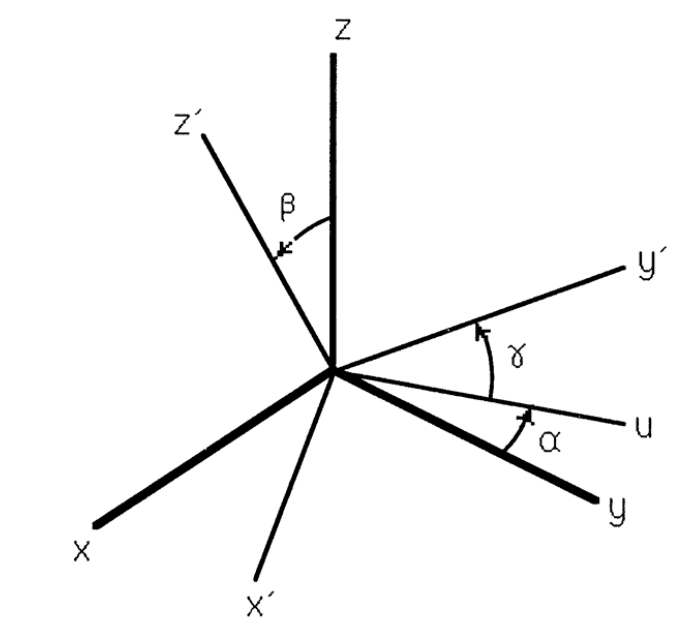
\includegraphics[height=4.5cm ,width=5cm]{QM/rotation.png}
	\caption{Euler angles}
\end{figure}
The net rotation is
\[\bm{R}(\alpha,\beta,\gamma) = \bm{R}_{z'}(\gamma) \bm{R}_{u}(\beta) \bm{R}_{z}(\alpha) = e^{-i\gamma J_{z'}} e^{-i\beta J_{u}} e^{-i\alpha J_{z}}\]
Since $J_u = \bm{R}_z(\alpha) J_y \bm{R}_z(-\alpha)$, we have $\bm{R}_u(\beta) = \bm{R}_z(\alpha) \bm{R}_y(\beta) \bm{R}_z(-\alpha)$. Similarly, we can obtain $\bm{R}_{z'}(\gamma) = \bm{R}_{u}(\beta) \bm{R}_z(\gamma) \bm{R}_u(-\beta)$. So, the rotation operator is
\[\bm{R}(\alpha,\beta,\gamma) = \bm{R}_{z}(\alpha) \bm{R}_{y}(\beta) \bm{R}_{z}(\gamma) = e^{-i\alpha J_{z}} e^{-i\beta J_{y}} e^{-i\gamma J_{z}}\]
The matrix representation of the rotation operator in the basis $|j,m\rangle$
\[\langle j',m' | \bm{R}(\alpha,\beta,\gamma) | j,m \rangle = \delta_{jj'} D_{m'm}^{(j)}(\alpha,\beta,\gamma)\]
gives rise to the rotation matrices,
\[D_{m'm}^{(j)}(\alpha,\beta,\gamma) = \langle j',m' | e^{-i\alpha J_{z}} e^{-i\beta J_{y}} e^{-i\gamma J_{z}} | j,m \rangle = e^{-i(\alpha m' + \gamma m)} d_{mm'}^{(j)}(\beta)\]
where
\[ d_{mm'}^{(j)}(\beta) = \langle j',m' | e^{-i\beta J_{y}} | j,m \rangle\]
For the case of $j = \frac{1}{2}$, we have $J_y = \frac{1}{2}\sigma_y$ and $\sigma_y^2 = I$. We can obtain
\[d^{(1/2)}(\beta) = \left[ \begin{matrix} \cos \frac{\beta}{2} & -\sin \frac{\beta}{2} \\ \cos \frac{\beta}{2}& \sin \frac{\beta}{2}\end{matrix} \right] \]
Notice that this matrix is periodic in $\beta$ with period $4\pi$, but it changes sign when $2\pi$ is added to $\beta$. This double-valuedness under rotation by $2\pi$ is a characteristic of the full rotation matrix whenever $j$ is a half odd-integer. The matrix is single-valued under rotation by $2\pi$ whenever $j$ is an integer.\\
Rotation of angular momentum eigenvectors now can be written as
\[\bm{R}(\alpha,\beta,\gamma)|j,m\rangle = \sum_{m'} D_{m'm}^{(j)}(\alpha,\beta,\gamma) |j,m'\rangle\]
When it comes to spherical harmonics, we have
\[Y_l^m(\theta',\phi') = \bm{R}^{-1}((\alpha,\beta,\gamma)) Y_l^m(\theta,\phi) = \sum_{m'} Y_{l}^{m'}(\theta,\phi) [D_{mm'}^{(j)}((\alpha,\beta,\gamma))]^*\]
By putting $\beta = \gamma = 0$ we obtain
\[Y_l^m(\theta,\phi+\alpha) = \sum_{m'} Y_{l}^{m'}(\theta,\phi) [D_{mm'}^{(j)}((\alpha,0,0))]^* = e^{i\alpha m} Y_{l}^{m}(\theta,\phi)\]
Setting $\phi=0$ then yields
\[Y_l^m(\theta,\alpha) = e^{i\alpha m} Y_{l}^{m}(\theta,0)\]
Since the direction $\theta = 0$ is the polar axis, continuity of the spherical harmonic requires that $Y_l^m(0,\alpha)$ be independent of $\alpha$. Therefore we must
have $Y_l^m(0,0) = 0$ for $m \neq 0$, and so we can write\\
\[Y_{l}^{m}(\theta,0) = c_{l}\delta{m0}\]
The we have
\[Y_l^m(\theta,\phi) = \sum_{m'} Y_{l}^{m'}(0,0) [D_{mm'}^{(j)}((\phi,\theta,\gamma))]^* = c_l [D_{m0}^{(j)}((\phi,\theta,\gamma))]^*\]
for arbitrary $\gamma$, thus obtaining a simple relation between the spherical harmonics and the rotation matrices. Conventional normalization is obtained if we put
\[c_l = \left( \frac{2l+1}{4\pi} \right) ^{1/2}\]
\\
The operator for a rotation through $2\pi$ about an axis
along the unit vector $\bm{n}$ is $\bm{R}_n(2\pi) = e^{-2\pi i\bm{n}\cdot\bm{J}}$. Its effect on the standard angular momentum eigenvectors is
\[\bm{R}_n(2\pi) = (-1)^{2j}|j,m\rangle \]
We assume a rotation through $2\pi$ as a trivial operation that leaves everything unchanged, i.e. all dynamical variables are invariant under $2\pi$ rotation:
\[\bm{R}(2\pi) A \bm{R}^{-1}(2\pi) = A\]
where $A$ may represent any physical observable. \\
the operator $\bm{R}_{2\pi}$ divides the vector space into two subspaces. A typical vector in the first subspace,
denoted as $|+\rangle$, has the property $\bm{R}(2\pi)|+\rangle = |+\rangle$, whereas a typical vector in the second subspace, denoted as $|-\rangle$, has the property $\bm{R}(2\pi)|-\rangle = -|-\rangle$. Now, if $A$ represents any physical observable, we have $\langle + | \bm{R}(2\pi) A| - \rangle = \langle + | A\bm{R}(2\pi)| - \rangle$, leading to 
\[\langle + | A | - \rangle = 0\] 
No physical observable can have nonvanishing matrix elements between states with integer angular momentum and states with half odd-integer angular momentum. This fact forms the basis of a superselection rule: There is no observable distinction among the state vectors of the form\\
\[|\Psi_{\omega}\rangle = |+\rangle + e^{i\omega}|-\rangle\]
for different values of the phase $\omega$.

\section{Addition of angular momentum}
Let us consider a two-component system, each component of which has angular momentum degrees of freedom. Basis vectors for the composite system can be formed from the basis vectors of the components by taking all binary products of a vector from each set
\[|j_1,j_2,m_1,m_2\rangle = |j_1,m_1\rangle ^{(1)} |j_2,m_2\rangle ^{(2)}\]
These vectors are common eigenvectors of the four commutative operators $\bm{J}^{(1)}\cdot\bm{J}^{(1)}$, $\bm{J}^{(2)}\cdot\bm{J}^{(2)}$, $\bm{J}_z^{(1)}$, and $\bm{J}_z^{(2)}$.
It is often desirable to form eigenvectors of the total angular momentum operators, $\bm{J}\cdot\bm{J}$ and $\bm{J}_z$, where the total angular momentum vector operator is
\[\bm{J} = \bm{J}^{(1)}\otimes\bm{1} + \bm{1}\otimes\bm{J}^{(2)}\]
This is useful when the system is invariant under rotation as a whole, but not under rotation of the two components separately. 
The eigenvectors of $\bm{J}\cdot\bm{J}$ and $\bm{J}_z$ may be denoted as $|\alpha, J, M \rangle$. It is easy to verify that the four operators $\bm{J}^{(1)}\cdot\bm{J}^{(1)}$, $\bm{J}^{(2)}\cdot\bm{J}^{(2)}$, $\bm{J}\cdot\bm{J}$ and $\bm{J}_z$ are mutually commutative, and hence they possess a complete set of common eigenvectors. 
Since the set of product vectors and the new set of total angular momentum eigenvectors are both eigenvectors of $\bm{J}^{(1)}\cdot\bm{J}^{(1)}$ and $\bm{J}^{(2)}\cdot\bm{J}^{(2)}$, the eigenvalues $j_1$ and $j_2$ will be constant in both sets. Therefore
we may confine our attention to the vector space of dimension $(2j_1+1)(2j_2+1)$ that is spanned by product vectors with fixed values of $j_1$ and $j_2$.\\
Now the $2J+1$ vectors $|\alpha, J, M \rangle$, with $M$ in the range $-J \leq M \leq J$, span an irreducible subspace.
Therefore if the vector $|\alpha, J, M \rangle$, for a particular value of $M$, can be constructed in the space under consideration, then so can the entire set of $2J+1$
such vectors with $M$ in the range $-J \leq M \leq J$.
For a particular value of $J$, it might be possible to construct one such set of vectors, two or more linearly independent sets, or none at all. \\
Let $N(J)$ denote the number of independent sets that can be constructed. Let $n(M)$ be the degree of degeneracy, in this space, of the eigenvalue $M$ . The relation between these two quantities is
\[n(M) = \sum_{J \geq |M|} N(J)\]
and hence
\[N(J) = n(J) - n(J+1)\]
The product vectors $|j_1,m_1\rangle |j_2,m_2\rangle$ are eigenvectors of the operator $\bm{J}_z$, with eigenvalue $m_1+m_2$, and the degree of degeneracy $n(M)$ is equal to the number of pairs $(m_1,m_2)$ such that $M=m_1+m_2$.
\begin{figure}[!h]
	\centering
	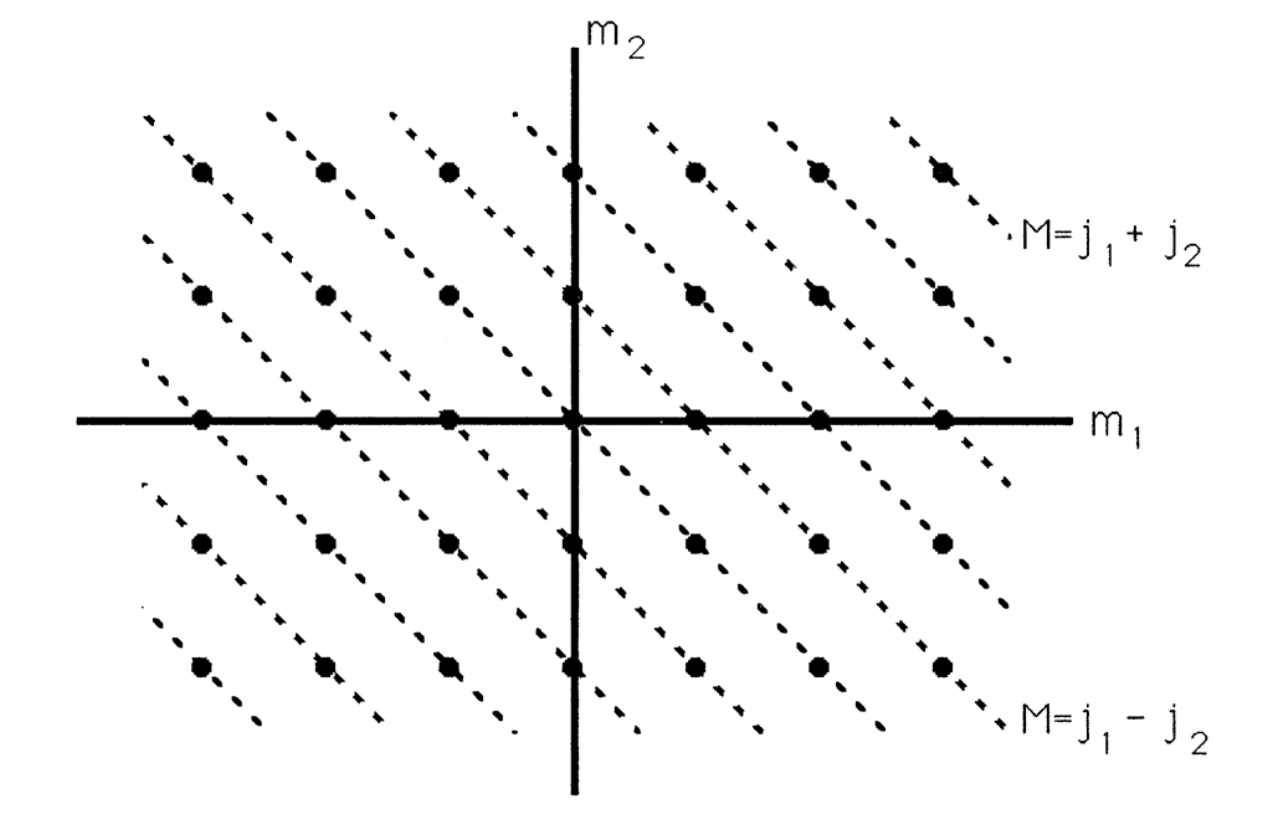
\includegraphics[height=4.14cm ,width=6.4cm]{QM/angular_momentum.png}
	\caption{Possible values of $M=m_1+m_2$ , illustrated for $j_1=3$, $j_2=2$}
\end{figure}
Therefore,
\[n(M)=\begin{cases} 0 \quad |M| > j_1 + j_2\\ j_1+j_2+1-|M|\quad |j_1-j_2| \leq M \leq |j_1+j_2|\\ 2j_{min}+1 \quad 0 \leq |M|\leq |j_1-j_2|\end{cases} \]
It then follows that
\[N(J)=\begin{cases} 1 \quad |j_1-j_2| \leq J \leq |j_1+j_2|\\ 0 \quad \mbox{otherwise}\end{cases} \]
It has turned out that $N(J)$ is never greater that $1$, and so the vectors $|\alpha, J, M \rangle$ can be uniquely labelled by the eigenvalues of the four operators $\bm{J}^{(1)}\cdot\bm{J}^{(1)}$, $\bm{J}^{(2)}\cdot\bm{J}^{(2)}$, $\bm{J}\cdot\bm{J}$ and $\bm{J}_z$. Henceforth these total angular momentum
eigenvectors will be denoted as $|j_1,j_2,J,M\rangle$. And we have the unitarity transformation 
\[|j_1,j_2,J,M\rangle = \sum_{m_1,m_2} |j_1,j_2,m_1,m_2\rangle \langle j_1,j_2,m_1,m_2 | j_1,j_2,J,M\rangle\]
The coefficients of this transformation are called the Clebsch–Gordan coefficients, denoted as $(j_1,j_2,m_1,m_2|J,M)$.
The phases of the CG coefficients are not yet defined because of the indeterminacy of the relative phases of the vectors $|j_1,j_2,J,M\rangle$. For different values of $M$ but fixed $J$ we adopt the usual phase convention that led to
\[J_+ |j_1,j_2,J,M\rangle = \sqrt{(J+M+1)(J-M)} |j_1,j_2,J,M+1\rangle\]
This leaves one arbitrary phase for each $J$ value, which we fix by requiring that $(j_1,j_2,j_1,J-j_1|J,J)$ be real and positive. It can be shown that all of the CG coefficients are now real.\\
We can also prove that the CG coefficient vanishes unless the following conditions are satisfied:
\begin{itemize}
\item $m_1+m_2=M$
\item $|j_1-j_2| \leq J \leq |j_1+j_2|$
\item $j_1+j_2+J =$ an integer
\end{itemize}
It is possible to calculate the values of the CG coefficients by successive application of the raising or lowering operator to
\[|j_1,j_2,J,M\rangle = \sum_{m_1,m_2} |j_1,j_2,m_1,m_2\rangle (j_1,j_2,m_1,m_2|J,M)\]
The details of the calculation can be found in section 7.7 of \emph{Quantum mechanics - a modern development(Leslie E. Ballentine)}.And we have \href{https://en.wikipedia.org/wiki/Table_of_Clebsch-Gordan_coefficients}{Table of CG coefficients} and \href{http://www.wolframalpha.com/input/?i=CG+coefficient}{Calculator of CG coefficients} on the internet. A special case of angular momentum addition is spin–orbit coupling of spin $\frac{1}{2}$ particles, and we list the corresponding CG coefficients $(l,\frac{1}{2}, M-m_s, m_s|J,M)$ in the table 1.1.
\begin{table}[!th]
\centering
\begin{tabular}{|c|c|c|}
\hline
 & $J=l+\frac{1}{2}$ & $J=l-\frac{1}{2}$ \\
 \hline
 $m_s = \frac{1}{2}$ & $\left[ \frac{l+M+\frac{1}{2}}{2l+1}\right ]^{\frac{1}{2}} $ & $-\left[ \frac{l-M+\frac{1}{2}}{2l+1}\right ]^{\frac{1}{2}} $ \\
 \hline
 $m_s = -\frac{1}{2}$ & $\left[ \frac{l-M+\frac{1}{2}}{2l+1}\right ]^{\frac{1}{2}} $ & $\left[ \frac{l+M+\frac{1}{2}}{2l+1}\right ]^{\frac{1}{2}} $ \\
\hline
\end{tabular}
\caption{Spin-Orbit coupling}
\end{table}\\
Now let us consider the relation between CG coefficients and rotation matrices. On the one hand, we have
\[\langle j_1,j_2,m_1,m_2 | \bm{R} | j_1,j_2,m'_1,m'_2\rangle = D_{m_1m'_1}^{(j_1)}(R) D_{m_2m'_2}^{(j_2)}(R)\]
On the other hand, we have
\begin{eqnarray}
&\phantom{=}& \langle j_1,j_2,m_1,m_2 | \bm{R} | j_1,j_2,m'_1,m'_2\rangle \nonumber \\
&=& \sum_{J,M,J',M'} (j_1,j_2,m_1,m_2|J,M) (j_1,j_2,m'_1,m'_2|J',M')  \langle j_1,j_2,J,M | \bm{R} | j_1,j_2,J',M'\rangle \nonumber \\
&=& \sum_{J,M,M'} (j_1,j_2,m_1,m_2|J,M) (j_1,j_2,m'_1,m'_2|J,M')D_{MM'}^{(J)}(R) \nonumber
\end{eqnarray}
So, we can get
\[D_{m_1m'_1}^{(j_1)}(R) D_{m_2m'_2}^{(j_2)}(R) = \sum_{J,M,M'} (j_1,j_2,m_1,m_2|J,M) (j_1,j_2,m'_1,m'_2|J,M')D_{MM'}^{(J)}(R)\]
It is called Clebsch-Gordan series.\\
Recall that
\[Y_l^m(\theta,\phi) =  \left( \frac{2l+1}{4\pi} \right) ^{1/2} [D_{m0}^{(j)}((\phi,\theta,0))]^* \]
so, we have
\[Y_{l_1}^{m_1}(\theta,\phi) Y_{l_2}^{m_2}(\theta,\phi) = \sum_{l,m} \sqrt{\frac{(2l_1+1)(2l_2+1)}{4\pi(2l+1)}} (l_1,l_2,m_1,m_2|l,m) (l_1,l_2,0,0|l,0) Y_l^m(\theta,\phi)\]
The orthogonal relation of spherical harmonics then would imply that
\[\int d\Omega Y_l^{m*}(\theta,\phi)Y_{l_1}^{m_1}(\theta,\phi) Y_{l_2}^{m_2}(\theta,\phi) = \sqrt{\frac{(2l_1+1)(2l_2+1)}{4\pi(2l+1)}} (l_1,l_2,m_1,m_2|l,m) (l_1,l_2,0,0|l,0)\]

\section{Tensor operators}
Suppose the state of the system is $|\psi\rangle$, then the state after rotation $R$ is $U(R)|\psi\rangle$, denoted as $|\psi'\rangle$. An operator $K$ is called scalar operator if and only if
\[\langle \psi' | K | \psi' \rangle = \langle \psi | K | \psi\rangle\]
i.e.
\[U^{-1}(R)KU(R) = K\]
Taking the case of infinitesimal rotation, we can derive that
\[[\bm{J},K] = 0\]
A group of operators $\bm{V}$ is called vector operator if and only if
\[\langle \psi' | V_i | \psi' \rangle = R_{ii'} \langle \psi | V_{i'} | \psi\rangle\]
i.e.
\[U^{-1}(R)V_{i}U(R) = \sum_{i'} R_{ii'} V_{i'}\]
Taking the case of infinitesimal rotation, we can derive that
\[[J_i, V_j] = i\epsilon_{ijk}V_k\]
If $\bm{V}$ and $\bm{W}$ are vector operators, we can prove that $\bm{V} \cdot \bm{W}$ is scalar operator and $\bm{V} \times \bm{W}$ is vector operator.\\
Similarly, tensor operators are defined as
\[U^{-1}(R) T_{ij\cdots k} U(R) = \sum_{i'\cdots} R_{ii'} R_{jj'} \cdots R_{kk'} T_{i'j'\cdots k'}\]
Such a tensor is known as a Cartesian tensor.\\
The trouble with a Cartesian tensor is that it is reducible, i.e. it can be decomposed into objects that transform independently under rotations. For example, the trace of a tensor transform like a scalar under rotations. 
So we now define spherical tensor operators which are irreducible under rotations.  We define a spherical tensor operator of rank $k$ with $(2k+1)$ components as
\[U^{-1}(R) T^{(k)}_q U(R) = \sum_{q'=-k}^{k} [D^{(k)}_{qq'}(R)]^* T^{(k)}_{q'}\]
or equivalently
\[U(R) T^{(k)}_q U^{-1}(R) = \sum_{q'=-k}^{k} D^{(k)}_{q'q}(R) T^{(k)}_{q'}\]
where $D^{(k)}_{qq'}$ is the rotation matrix.\\
Taking the case of infinitesimal rotation, we can derive that
\[[J_{\pm},T^{(k)}_{q}] = \sqrt{(k \mp q)(k \pm q +1)} T^{(k)}_{q \pm 1}\]
\[[J_z, T^{(k)}_{q}] = q T^{(k)}_{q}\]
For example, spherical components of a vector operator $\bm{V}$, 
\[V_{-1} = \frac{V_x - i V_y}{\sqrt{2}} \quad V_0 = V_z \quad V_{1} = -\frac{V_x + i V_y}{\sqrt{2}}\]
satisfy the commutation relation above, so they are spherical tensor of rank $1$. Generally, if $\bm{V}$ is a vector operator, then $Y_l^m(\bm{V})$ is a spherical tensor of ranks $l$.\\
Spherical tensors can be formed as products of other spherical  tensors, we have following theorem.\\

\begin{newthem}
Let $X^{(k_1)}_{q_1}$ and $Z^{(k_2)}_{q_2}$ be irreducible spherical tensors of rank $k_1$ and $k_2$. Then
\[T^{(k)}_{q} = \sum_{q_1.q_2} (k_1,k_2,q_1,q_2|k,q) X^{(k_1)}_{q_1} Z^{(k_2)}_{q_2}\]
is a irreducible spherical tensor of rank $k$. 
\end{newthem}
\noindent
The proof can be found in section 3.10 of \emph{Modern Quantum Mechanics(J.J.Sakurai)}.\\
For example, suppose $\bm{V}$ and $\bm{U}$ are spherical tensor
\[T^{(0)}_{0} = \sqrt{\frac{1}{3}} (U_{-1}V_{1} + U_{1}V_{-1}-U_{0}U_{0}) = - \sqrt{\frac{1}{3}} (U_x^2 + U_y^2 + U_z^2)\]
is tensor of rank $1$, then is a spherical tensor of rank $0$. Another important theorem is Wigner-Eckart theorem.\\

\begin{newthem}[Wigner-Eckart theorem]
The matrix elements of tensor operators with respect to angular-momentum eigenstates satisfy
\[\langle \tau',j',m'| T^{(k)}_{q}| \tau,j,m\rangle = (j,k,m,q|j',m') \frac{\langle \tau',j' || T^{(k)} || \tau,j\rangle}{\sqrt{2j+1}}\]
where the double-bar matrix element is independent of $m$ and $m'$ and $q$.
\end{newthem}
\noindent
The proof can be found in section 3.10 of \emph{Modern Quantum Mechanics(J.J.Sakurai)}.\\
So, for scaler operator $K$, we have
\[\langle \tau',j',m'| S| \tau,j,m\rangle = \delta_{jj'}\delta_{mm'} \frac{\langle \tau',j' || S || \tau,j\rangle}{\sqrt{2j+1}}\]
For spherical tensor of rank $1$, we have
\[\langle \tau',j',m'| V_{q} | \tau,j,m\rangle = (j,1,m,q|j',m') \frac{\langle \tau',j' || V_q || \tau,j\rangle}{\sqrt{2j+1}}\]
It would vanish unless
\[m'-m = q \quad j'-j = 0,1,-1 \quad j \mbox{ and } j' \mbox{ are not both  } 0\]
For $j=j'$, Wigner-Eckart theorem - when applied to the vector operator- takes a particularly simple form. We can derive that
\[\langle \tau',j,m' | V_q | \tau, j ,m \rangle = \frac{\langle \tau',j,m | \bm{J}\cdot\bm{V} | \tau, j ,m \rangle}{j(j+1)} \langle j,m' | J_q | j ,m \rangle\]
For example, the magnetic moment operator for an atom has the form
\[\bm{\mu} = \frac{-e}{2m_e } (g_L\bm{L} + g_s \bm{S})\]
The parameters $g_L$ and $g_S$ have approximately the
values $g_L = 1$ and $g_S = 2$. The former is an generalization of the magnetic moment we calculated in classical electrodynamics for a system of charged particles. The latter will be discussed in quantum field theory.
We define the effective Lande factor as
\[\langle \tau,J,M' | \bm{\mu} | \tau,J,M \rangle = \frac{-e}{2m_e } g_{eff} \langle J,M' | \bm{J} | J,M \rangle\]
Then, we have
\[g_{eff} = \frac{\langle \tau,J,M | g_L\bm{L}\cdot\bm{J} + g_s \bm{S}\cdot\bm{J} | \tau,J,M \rangle}{J(J+1)} = 1 + \frac{J(J+1)- L(L+1) + S(S+1)}{2J(J+1)}\]

\section{Spherical potential well}
The stationary states of a particle in the spherical potential well are determined by
\[-\frac{1}{2m}\nabla^2 \Psi  + W(r) \Psi = E\Psi \]
In spherical coordinates, 
\[\nabla^2 = \frac{1}{r^2} \frac{\partial}{\partial r} \left [ r^2\frac{\partial}{\partial r} \right ] + \frac{1}{r^2\sin\theta} \frac{\partial}{\partial \theta} \left [\sin\theta \frac{\partial}{\partial \theta} \right ] + \frac{1}{r^2\sin^2\theta} \frac{\partial^2}{\partial\phi^2}\]
So, the eigenvalue equation becomes
\[-\frac{1}{2m} \frac{1}{r^2} \frac{\partial}{\partial r} \left [ r^2\frac{\partial \Psi}{\partial r}\right ]  + \frac{L^2}{2Mr^2} \Psi + W(r)\Psi = E\Psi\]
Suppose the eigenfunctions have the factored form
\[\Psi(r,\theta,\phi) = Y_l^m(\theta,\phi) \frac{u(r)}{r}\]
The radial function then satisfies the equation
\[-\frac{1}{2m} \frac{d^2 u(r)}{dr^2} + \left[ \frac{l(l+1)}{2mr^2} + W(r)\right]u(r) = Eu(r)\]
The radial function must satisfy the boundary condition $u(0) = 0$ since $\Psi(r,\theta,\phi)$ would otherwise have an $r^{-1}$ singularity at the origin. The normalization $\langle \Psi | \Psi \rangle = 1$ implies that
\[\int_0^{\infty} = |u(r)|^2 dr = 1\]

\subsubsection{The hydrogen atom}
The hydrogen atom is a two-particle system consisting of an electron and a proton. The Hamiltonian is
\[H = \frac{P_e^2}{2m_e} + \frac{P_p^2}{2m_p} - \frac{e^2}{4\pi|\bm{Q}_e-\bm{Q}_p|}\]
We take as independent variables the center of mass and relative coordinates of the particles
\[\bm{Q}_c = \frac{m_e\bm{Q}_e + m_p\bm{Q}_p}{m_e+m_p} \quad \bm{Q}_r = \bm{Q}_e-\bm{Q}_p\]
The corresponding momentum operators are
\[\bm{P}_c = \bm{P}_e + \bm{P}_p \quad \bm{P}_r = \frac{m_p\bm{P}_e-m_e\bm{P}_p}{m_e + m_p}\]
We can verify that
\[[Q_{c\alpha},P_{c\beta}] = [Q_{r\alpha},P_{r\beta}] = i\delta_{\alpha\beta} \quad [Q_{c\alpha},P_{r\beta}] = [Q_{r\alpha},P_{c\beta}] = 0\]
The Hamiltonian becomes
\[H = \frac{P_c^2}{2(m_e+m_p)} + \frac{p_r^2}{2\mu} - \frac{e^2}{4\pi|\bm{Q}_r|}\]
where $\mu$ is called the reduced mass, and is defined by $\mu \equiv \frac{m_em_p}{m_e+m_p}$.
The center of mass behaves as a free particle, and its
motion is not coupled to the relative coordinate. We shall confine our attention to the internal degrees of freedom described by the relative coordinate $\bm{Q}_r$. The energy eigenvalue equation in coordinate representation is
\[-\frac{1}{2\mu}\nabla^2 \Psi(\bm{r})  -\frac{e^2}{4\pi r} \Psi(\bm{r}) = E\Psi(\bm{r})\]
Suppose $\Psi(r,\theta,\phi) = Y_l^m(\theta,\phi) \frac{u(r)}{r}$, we have
\[-\frac{1}{2\mu} \frac{d^2 u(r)}{dr^2} + \left[ \frac{l(l+1)}{2\mu r^2} - \frac{e^2}{4\pi r}\right]u(r) = Eu(r)\]
Define
\[\rho \equiv \alpha r \quad \alpha \equiv \sqrt{8\mu|E|} \quad \lambda \equiv \frac{e^2}{4\pi} \sqrt{\frac{\mu}{2|E|}}\]
we have
\[\frac{d^2 u}{d\rho^2} + \left[ -\frac{1}{4} + \frac{\lambda}{\rho} - \frac{l(l+1)}{\rho^2} \right] u = 0\]
As $\rho \to \infty$, we have $u \sim e^{-\rho/2}$. And as $\rho \to 0$, we have $u \sim \rho^{l+1}$. So, we can suppose
\[u(\rho) = \rho^{l+1} e^{-\rho/2} v(\rho)\]
And we can get
\[\rho \frac{d^2 v}{d\rho^2} + (2l+2-\rho)\frac{dv}{d\rho} + (\lambda-l-1)v = 0\]
It is the so-called \href{http://mathworld.wolfram.com/ConfluentHypergeometricDifferentialEquation.html}{Confluent Hypergeometric Differential Equation}.
When $\lambda - 1- l = n_r$, we have regular solutions. Solutions are \href{https://en.wikipedia.org/wiki/Laguerre_polynomials#Generalized_Laguerre_polynomials}{Associated Laguerre Polynomial}, and will be denoted as $L_{n-l-1}^{2l+1}(\rho) (n=n_r+l+1)$. The energy levels are
\[E_n = -\frac{\mu e^4}{32\pi^2 n^2}\]
The degeneracy of an eigenvalue $E_n$ is
\[\sum_{l=0}^{n-1} (2l+1) = n^2\]
\begin{note}
The degeneracy of an energy level of a hydrogen atom is greater than this by a factor of $4$, which arises from the two-fold orientational degeneracies of the electron and proton spin states. This four-fold degeneracy is modified by the hyperfine interaction between the magnetic moments of the electron and the proton.
\end{note}
The orthonormal energy eigenfunctions for the hydrogen atom are
\[\Psi_{nlm}(r,\theta,\phi) =  \left[ \frac{4(n-l-1)!}{(na_0)^3 n[(n+l)!]^3} \right]^{\frac{1}{2}} \rho^l L_{n-l-1}^{2l+1}(\rho) e^{-\rho/2} Y_l^m (\theta,\phi)\]
where $\rho = \alpha r = \frac{2r}{na_0}$, and $a_0 \equiv \frac{4\pi}{\mu e^2}$ is a characteristic length for the
atom, known as the Bohr radius.The ground state wave
function is
\[\Psi_{000} = (\pi a_0^3)^{-\frac{1}{2}} e^{-\frac{r}{a_0}}\]
A measure of the spatial extent of the bound states of hydrogen is given by the averages of various powers of the distance $r$.
\begin{eqnarray}
\langle r \rangle &=& n^2a_0 \left \{ 1 + \frac{1}{2} \left [ 1 - \frac{l(l+1)}{n^2} \right] \right\} \nonumber \\
\langle r^2 \rangle &=& n^4a_0^2 \left \{ 1 + \frac{3}{2} \left [ 1 - \frac{l(l+1)-1/3}{n^2} \right] \right\} \nonumber \\
\langle \frac{1}{r} \rangle &=& \frac{1}{n^2 a_0} \nonumber
\end{eqnarray}
\end{document}
